These wireframe diagrams act as a simple mock-up of the graphical user interface that we have designed, showing the outline of the three main windows with which the user will interact. Although the Live Brief stated that the program can be designed for CLI (Command Line Interface), we have decided that having a simple GUI (Graphical User Interface) will be more intuitive and faster. The wireframe diagram reflects our focus on designing the GUI to be minimalistic and straightforward, requiring as few steps as possible in order to fulfil its functionality. 
\begin{figure}[h]
    \centering
    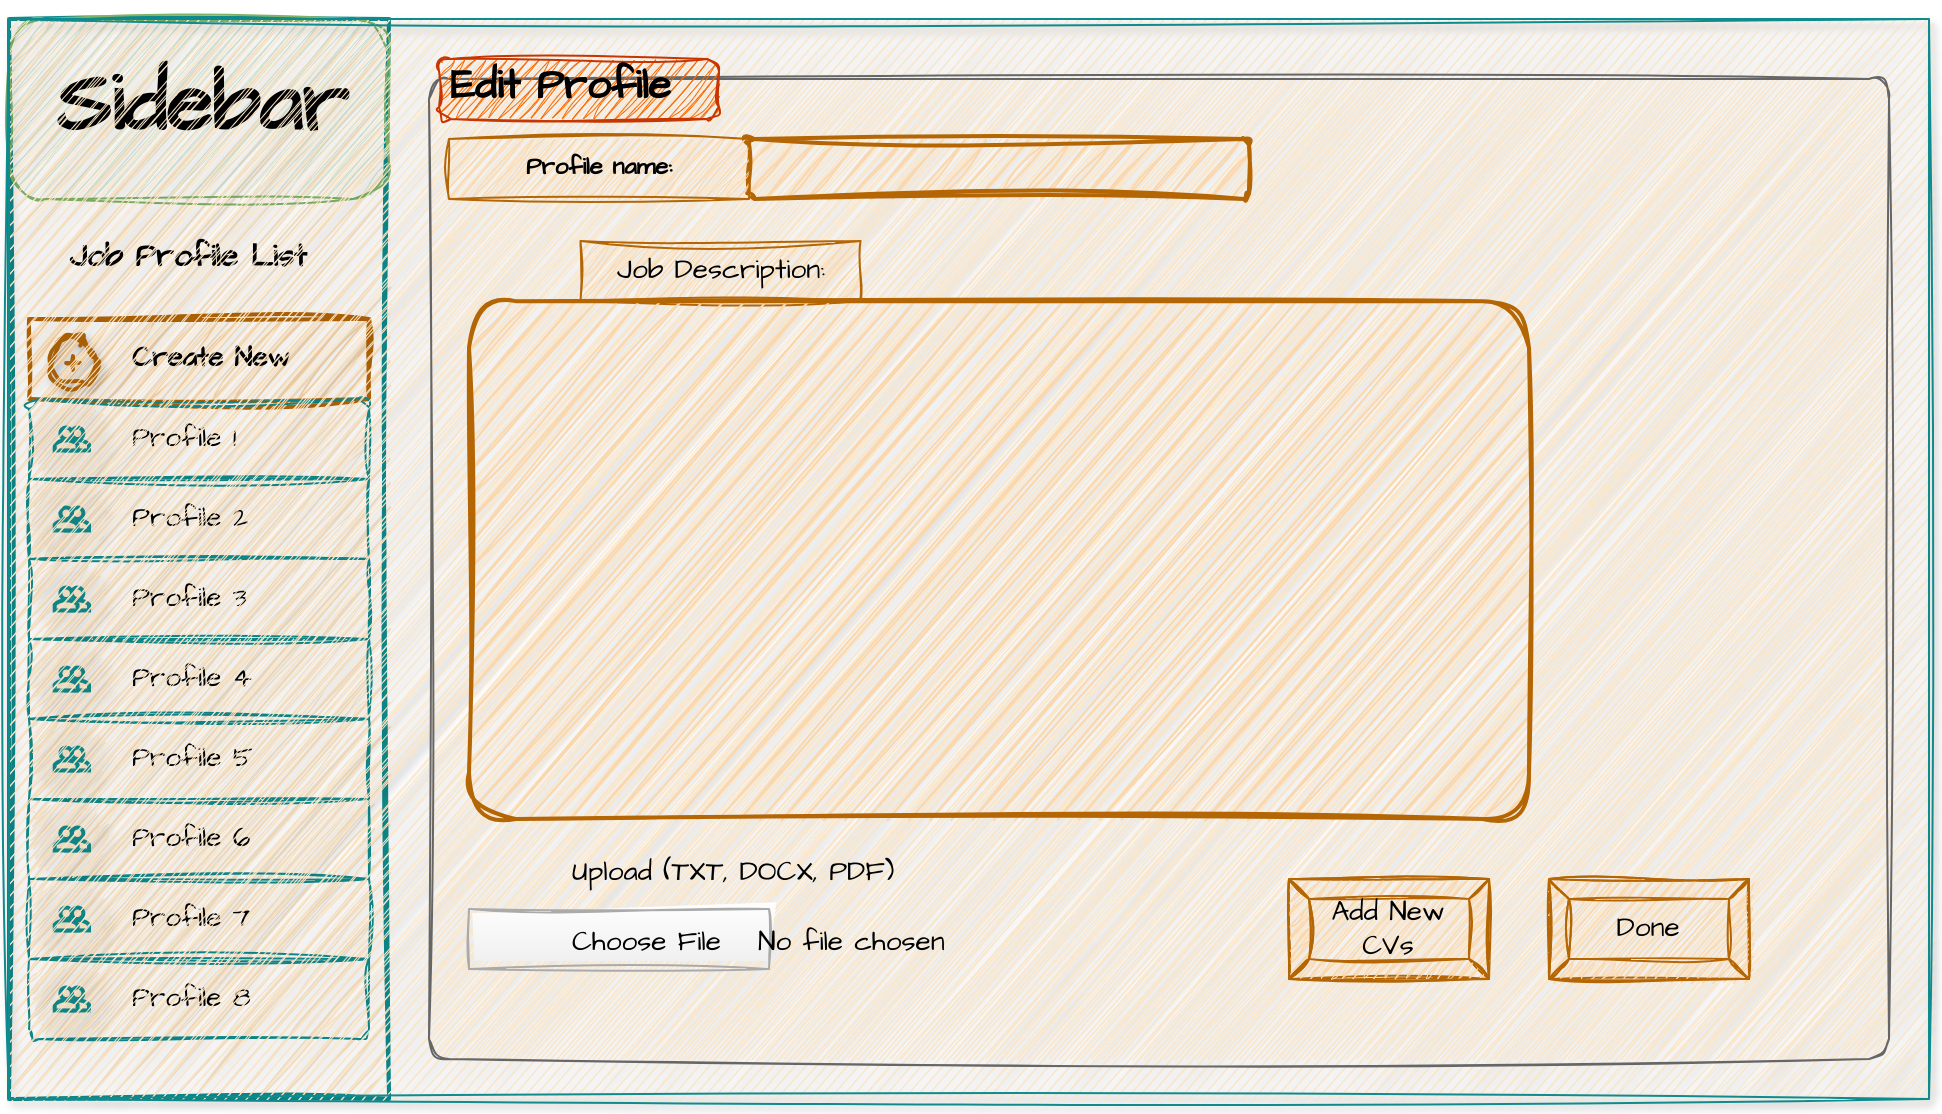
\includegraphics[width=1\linewidth]{img/wireframe/wireframeCreateProfile.drawio.png}
    \caption{"Edit Profile" acts as the the starting screen when the program is launched, or "New Profile" is selected. When "Edit Profile" is selected, the fields in this screen hold the relevant data rather than being empty. That way we simplify the UI by removing the need for separate "New Profile" and "Edit Profile" screens.}
\end{figure}
\begin{figure}[h]
    \centering
    \includegraphics[width=1\linewidth]{img/wireframe/wireframeProfile.drawio.png}
    \caption{The "Profile" screen displays a ranked list of job applicant CVs alongside their relevance score and relevant tags that match the job description's criteria.}
\end{figure}
\begin{figure}[h]
    \centering
    \includegraphics[width=1\linewidth]{img/wireframe/wireframeResumeView.drawio.png}
    \caption{Clicking on a CV on the list will bring up the "Resume" screen which allows the user to navigate through viewing individual CVs.}
\end{figure}
